\section{Experimental setup Calibration}

\subsection{Set-up}
Before performing the source spectra measurements, the detector was connected to the HV power supply and to an amplifying circuit consisting of a \textit{preamplifier} and a \textit{coarse-gain amplifier}, shown on respectively in figure \ref{fig:preamp_photo} and \ref{fig:ampli_gene}. 

\begin{figure}[ht]
  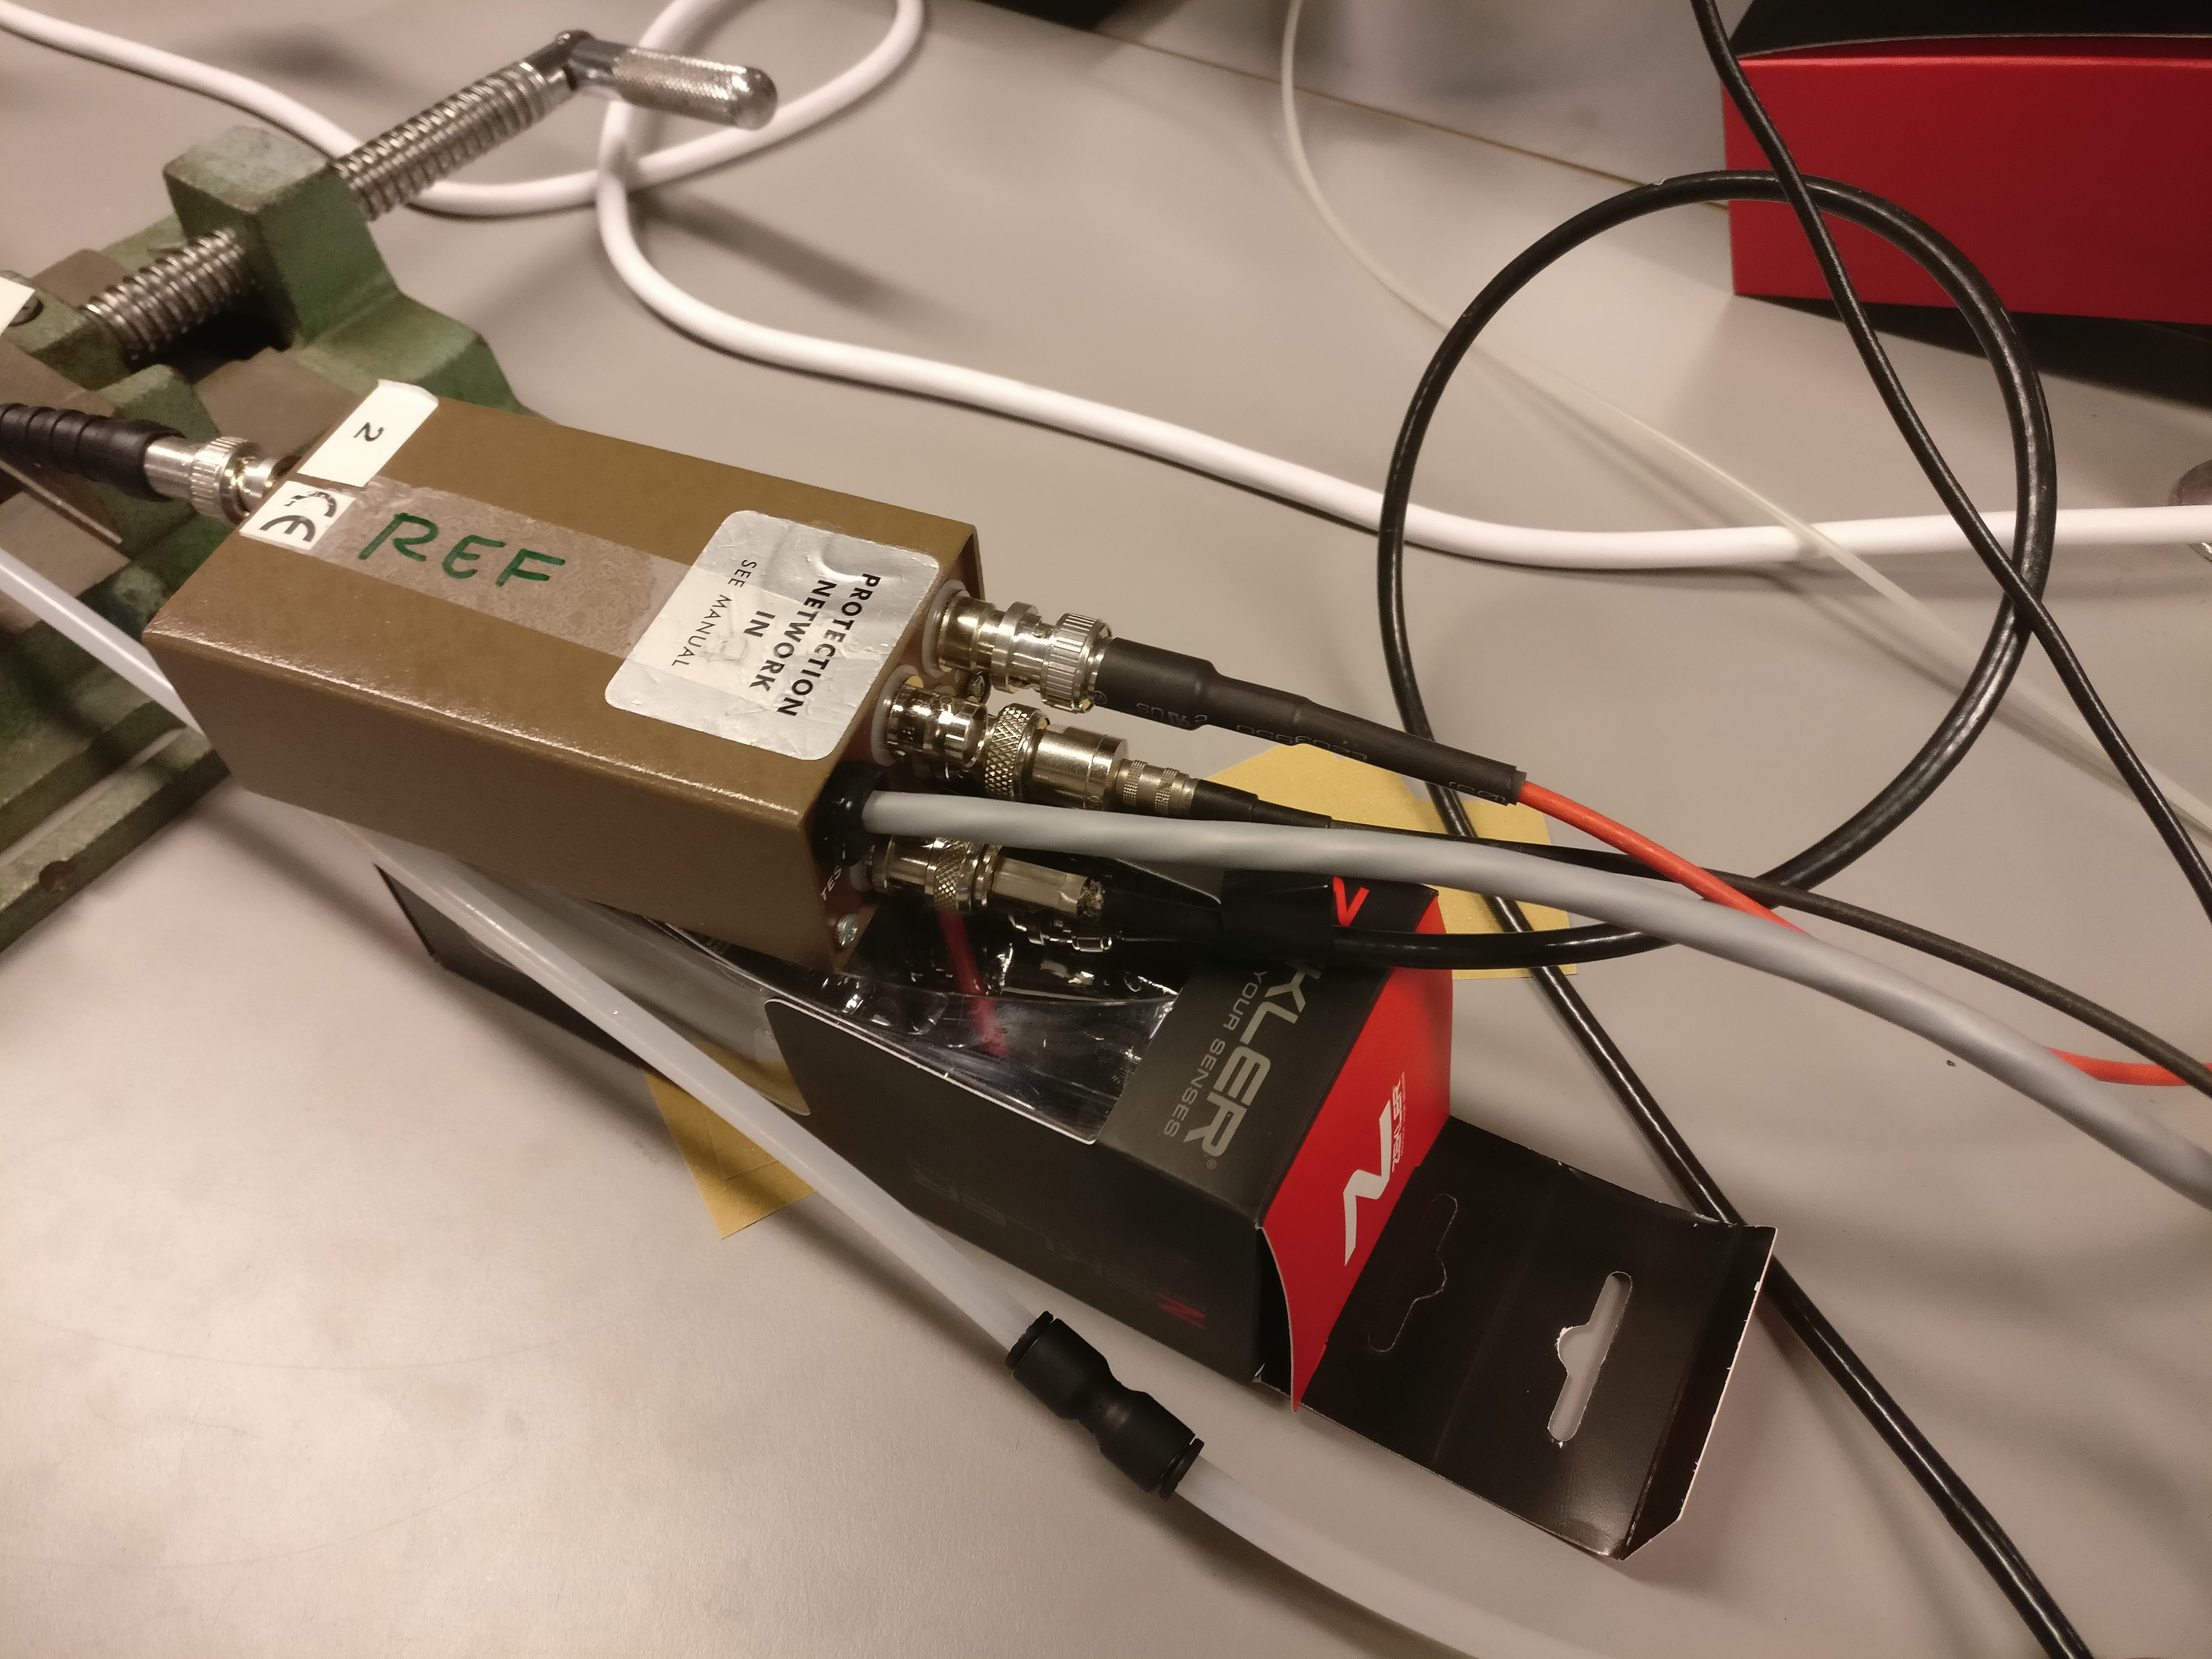
\includegraphics[width=\textwidth]{graphics/preamplifier.jpg}
  \caption{Photograph of the preamplifier unit.}
  \label{fig:preamp_photo}
\end{figure}

\begin{figure}[ht]
  \includegraphics[width=\textwidth]{graphics/amplifier_photo.jpg}
  \caption{Photograph of the pulse generator used to inject pulses into the preamplifer, and the coarse gain amplifier used in front of the MCA}
  \label{fig:ampli_gene}
\end{figure}

Both system contribute to increase the overall number of signal electrons collected per avalanche occuring in the drift chamber. The overall gain in signal, between the drift chamber electrode and the final Multi-Channel Analyzer (MCA) reading out data, is given by equation \ref{eq:gain_system}.

\begin{equation}
  \label{eq:gain_system}
  Q_{MCA} = Q_{drift}\cdot G_{pre}\cdot G_{coarse}
\end{equation}


\subsection{Calibration of the pre-amplifier gain}
 Calibrated pulses of various intensities were injected into the electronics, and the output was displayed onto an oscilloscope to evaluate the gain of the preamplifier, $G_{pre}$ and its uncertainty.


\begin{figure}[ht]
  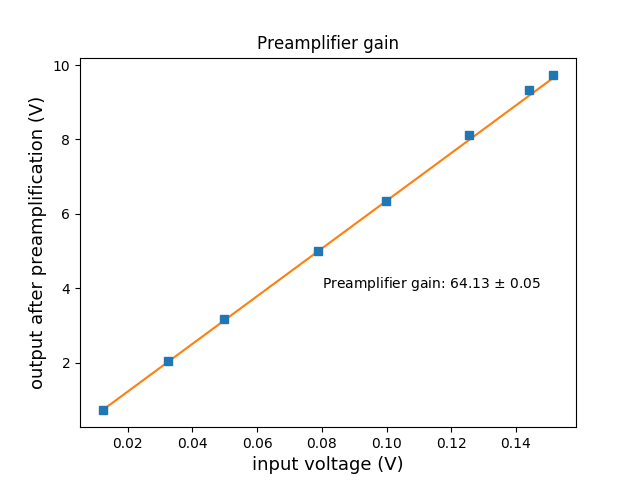
\includegraphics[width=\textwidth]{graphics/preamp_gain_calibration.png}
  \caption{Output voltage of pulses injected into the pre-amplifier electronics.}
  \label{fig:preamp_gain}
\end{figure}


\subsection{Calibration of the Coarse Gain amplifier}
To estimate the uncertainty on the coarse gain amplifier, subsequent runs of Fe$^{55}$ and Am$^{241}$ spectra acquisitions were made at the same operating voltage, but different coarse gain settings. Figure \ref{fig:coarse_gain} shows the result of this analysis. Since the data acquired only allowed us to measured \textit{ratios} of gain settings, the uncertainties of the absolute amplifier gain are simply assumed to scale with the lowest gain setting possible. In other words, the amplifier gain at a particular setting can be defined as:

\begin{equation}
  \label{eq:gain_abs}
  G_{coarse} = 2\cdot\Pi_{i>2}^{i=j}\frac{G_{i}}{G_{i-1}}
\end{equation}

where $j$ is the gain level at which the amplifier is operated. Figure \ref{fig:coarse_gain} presents the various ratios of gain settings measured, using both the Fe$^{55}$ and Am$^{241}$ source. The red data point show the result of combining both results, which allows us to get better estimates of the gain ratio uncertainties.

\begin{figure}[ht]
  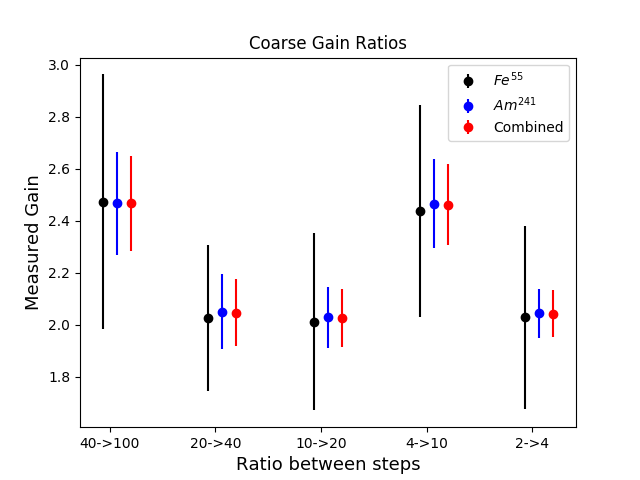
\includegraphics[width=\textwidth]{graphics/coarse_gain_calibration.png}
  \caption{Determination of the coarse gain amplification uncertainties. Results are presented in the form of gain ratios between every adjacent setting of the coarse gain knob. The combined value and uncertainty on each measurement is shown by the red data points.}
  \label{fig:coarse_gain}
\end{figure}


